\subsection{Figures}
\begin{figure}[!htb]
\centering
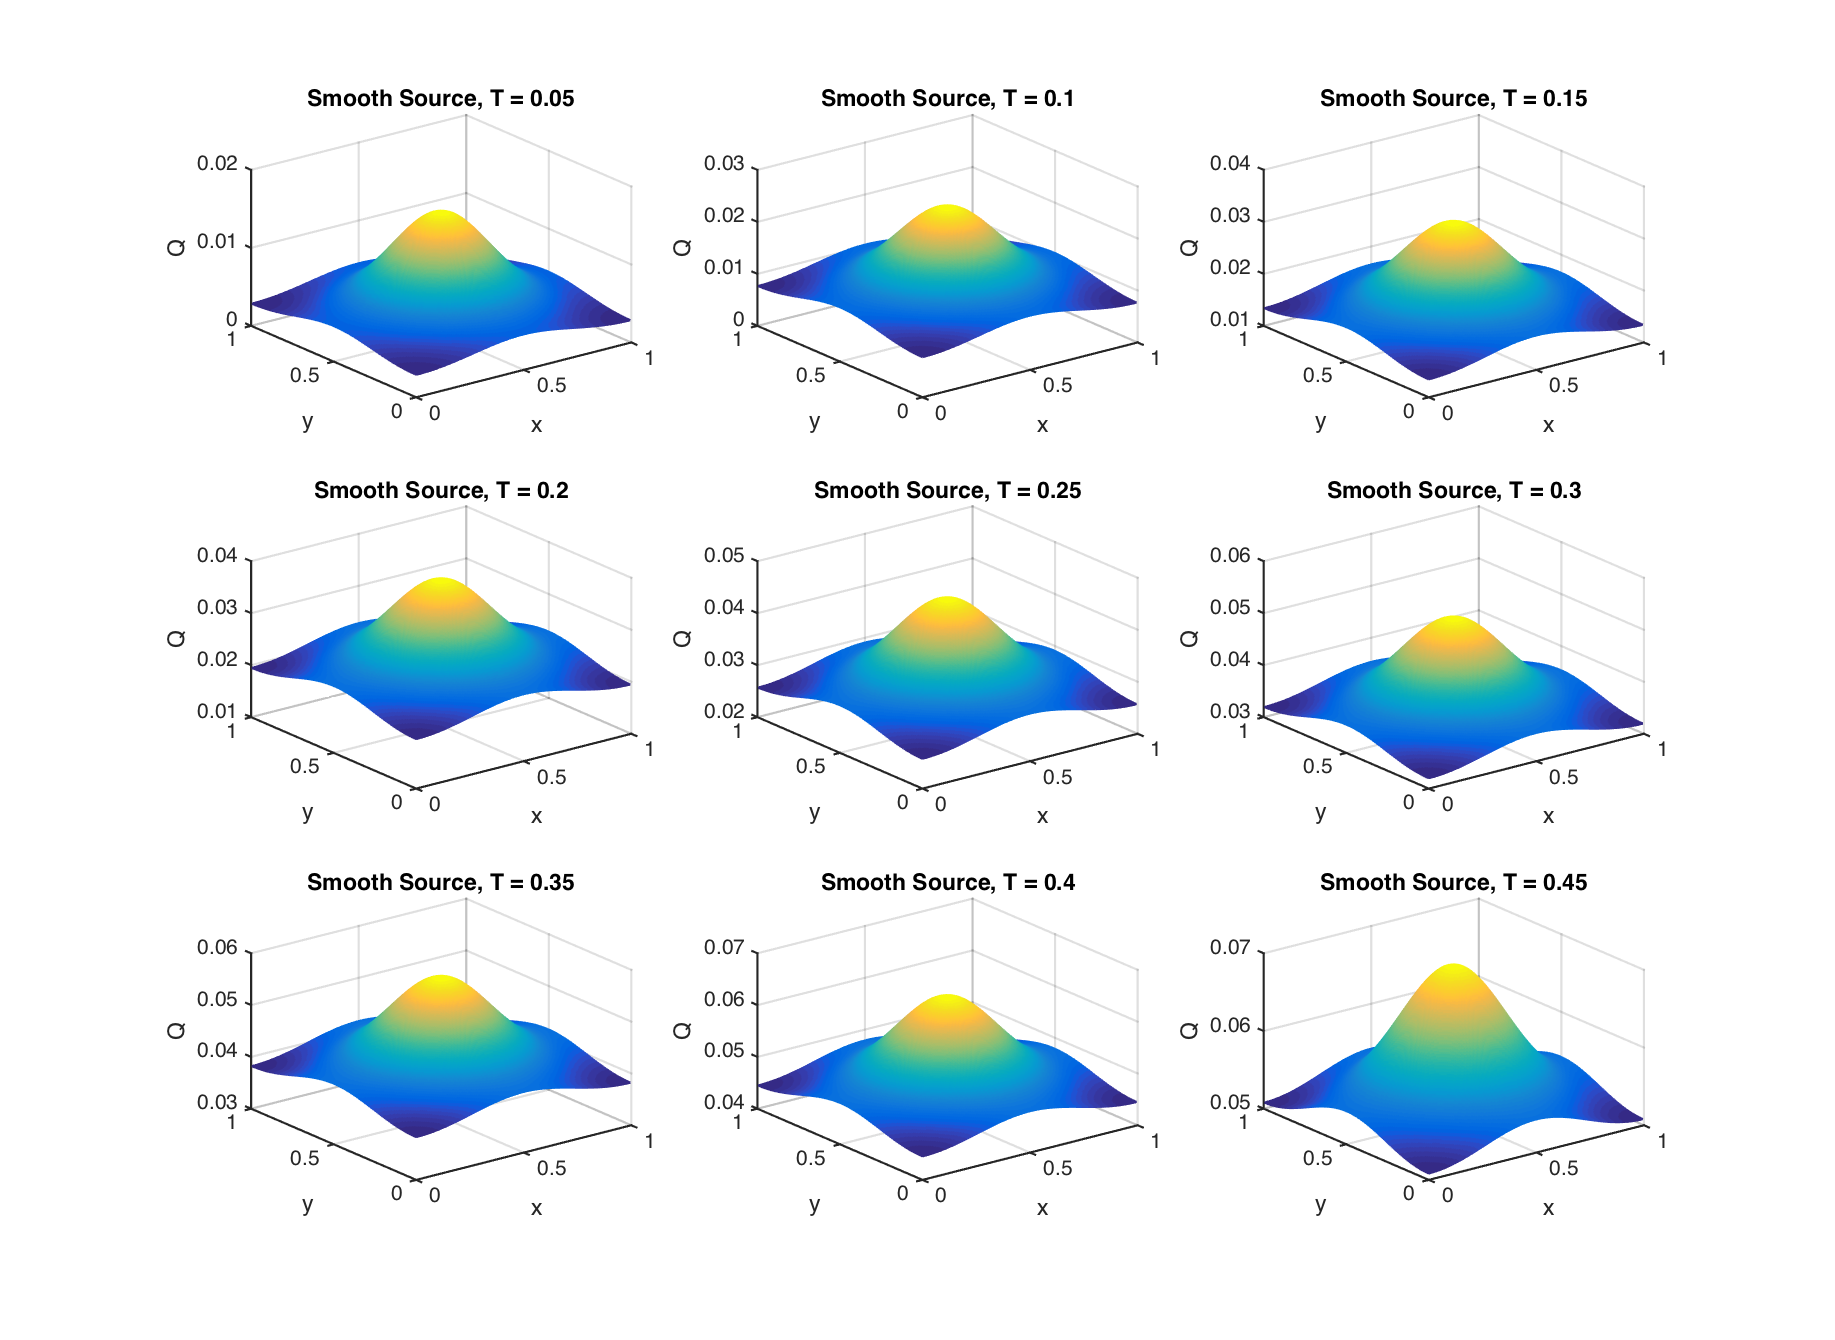
\includegraphics[scale=.5]{smoothSource4_1.eps}
\caption{}
\label{fig:digraph}
\end{figure}

\begin{figure}[!htb]
\centering
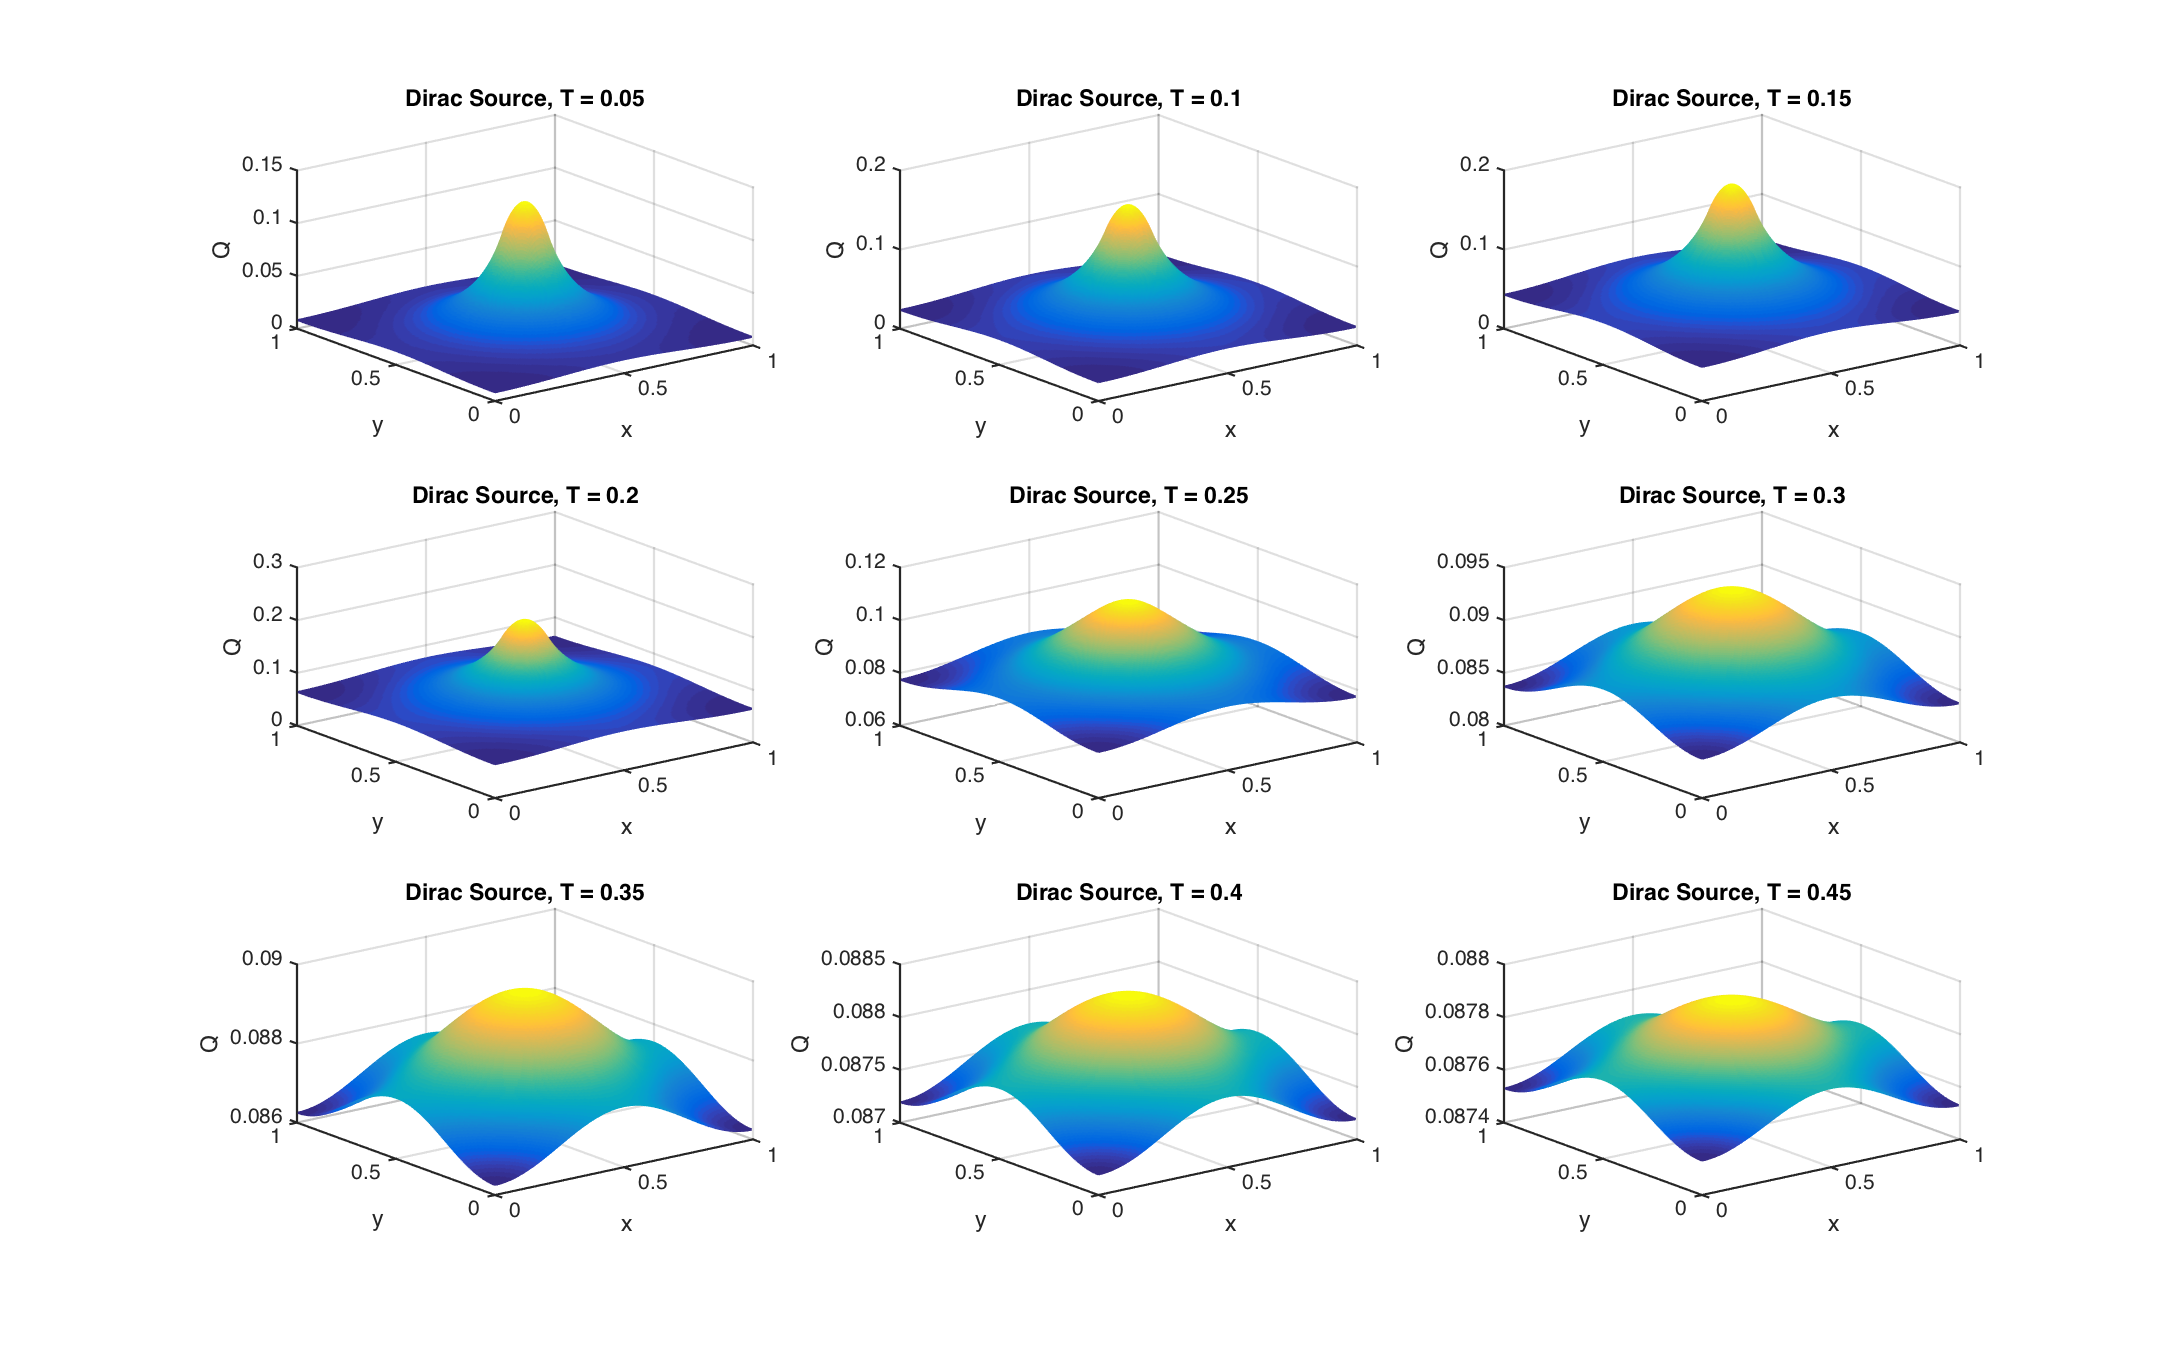
\includegraphics[scale=.5]{diracSource4_1.eps}
\caption{}
\label{fig:digraph}
\end{figure}

\subsection{Convergence}
Because we do not know the true solution to the problem, we study ratios, which we denote by $R$, of the differences of the computed values i.e. 
\begin{align*}
R=\frac{Q'_{h/2,t} - Q'_{h,t}}{Q'_{h/4,t} - Q'_{h/2,t}}
\end{align*}
where, for example, $Q'_{h/2,t}$ is our computed solution using $\Delta x = \Delta y = h/2$ and $\Delta t = t$. We wish to show that the error behaves as $O(\Delta t^p) + O(\Delta h^r)$ and find $p$ and $r$. Letting $Q*$ denote the true solution, we write write our ratio as  
\begin{align*}
R = \frac{Q*+O(\Delta t^p) + O(\Delta (h/2)^r) - (Q* + O(\Delta t^p) + O(\Delta h^r))}{Q*+O(\Delta t^p) + O(\Delta (h/4)^r) - (Q*+O(\Delta t^p) + O(\Delta (h/2)^r))} = \frac{O(\Delta (h/2)^r)-O(\Delta h^r)}{O(\Delta (h/4)^r) - O(\Delta (h/2)^r)}
\end{align*}
To get the order of convergence from $R$, we take the log base 2. This gives us 
\begin{align*}
log_2(R) &= log_2(\frac{O(\Delta (h/2)^r)-O(\Delta h^r)}{O(\Delta (h/4)^r) - O(\Delta (h/2)^r)}) \\ 
&= log_2(\frac{2^{-r}O(\Delta h^r)-O(\Delta h^r)}{2^{-r}(2^{-r}O(\Delta h^r)-O(\Delta h^r))}) \\
&= log_2(2^{r}) \\
&= r
\end{align*}
We compute several values of $log_2(R)$ using different h values. We get the following values
\begin{table}[]
\centering
\caption{Order of Convergence in h}
\label{my-label}
\begin{tabular}{|c|c|c|c|}
\hline 
 & h=0.025 & h=0.0125 & 0.00625 \\ 
\hline 
$log_2(R)$ & 1.9962 & 1.9990 & 1.9986 \\ 
\hline 
\end{tabular} 
\end{table}
from which we can infer that $r = 2$. We do the same thing in $t$ with
\begin{align*}
R = \frac{O(\Delta (t/2)^p)-O(\Delta t^p)}{O(\Delta (t/4)^p) - O(\Delta (t/2)^p)}
\end{align*} 
and obtain the following values
\begin{table}[]
\centering
\caption{Order of Convergence in h}
\label{my-label}
\begin{tabular}{|c|c|c|c|}
\hline 
 & $t=4x10^{-4}$ & $t=2x10^{-4}$ & $t=1x10^{-4}$ \\ 
\hline 
$log_2(R)$ & 1.0000 & 1.0000 & 1.0000 \\ 
\hline 
\end{tabular} 
\end{table}
from which we infer that $p=1$. This values are in agreement with numerical theory because the derivative with respect to time is computed with the first order Euler scheme, which has first order convergence, and second order finite difference for the second derivative with respect to time, which has second order convergence.   